\documentclass{article}
\usepackage{minted}
\usepackage[spanish]{babel}
\usepackage{hyperref}
\usepackage{graphicx}
\graphicspath{ {./images/} }

%%%%%%%%%%%%%%%%%%%%%%%%%%%%%%%%%%%%%%%%%%%%%%%%%%%%%%
% COMIENZA EL DOCUMENTO
%%%%%%%%%%%%%%%%%%%%%%%%%%%%%%%%%%%%%%%%%%%%%%%%%%%%%%

\begin{document}

\tableofcontents

\section{Túneles 6in4}
Dado el siguiente escenario:

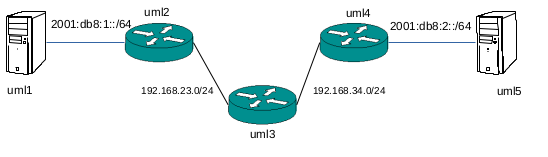
\includegraphics[width=\textwidth]{tuneles6in4}

\begin{minted}{bash}
  # net.conf
  defsw br12 uml1.0 uml2.0
  defsw br23 uml2.1 uml3.0
  defsw br34 uml3.1 uml4.0
  defsw br23 uml4.1 uml5.0
\end{minted}

\begin{minted}{lexer.py:IOSLexer -x}
  ! UML1 y UML5
  configure terminal
  int eth0
  no shutdown
  end
  write
\end{minted}

\begin{minted}{lexer.py:IOSLexer -x}
 ! UML2
 configure terminal
 int eth0
 ipv6 address 2001:db8:1::1/64
 ipv6 nd prefix 2001:db8:1::/64 ! Para que anuncie su prefijo a UML1
 no ipv6 nd suppress-ra
 quit
 int eth1
 ip address 192.168.23.1/24
 quit
 ip route 0.0.0.0/0 192.168.23.2
 ipv6 forwarding
 ip forwarding
 end
 write
\end{minted}

\begin{minted}{lexer.py:IOSLexer -x}
 ! UML3
 configure terminal
 int eth0
 ip address 192.168.23.2/24
 quit
 int eth1
 ip address 192.168.34.2/24
 quit
 ip forwarding
 ip route 192.168.23.0/24 192.168.34.2
 ip route 192.168.34.0/24 192.168.23.2
 end
 write
\end{minted}

\begin{minted}{lexer.py:IOSLexer -x}
 ! UML4
 configure terminal
 int eth0
 ip address 192.168.34.1/24
 quit
 int eth1
 ipv6 address 2001:db8:2::1/64
 ipv6 nd prefix 2001:db8:2::/64 ! Para que anuncie su prefijo a UML5
 no ipv6 nd suppress-ra 
 quit
 ip route 0.0.0.0/0 192.168.34.2
 ipv6 forwarding
 ip forwarding
 end
 write
\end{minted}

\begin{minted}{bash}
 # UML2 (bash)
 ip tunnel add tunnel1 mode sit remote 192.168.34.1
 ip link set dev tunnel1 up mtu 1400
 ip route add 2001:db8:2::/64 dev tunnel1
\end{minted}

\begin{minted}{bash}
 # UML4 (bash)
 ip tunnel add tunnel2 mode sit remote 192.168.23.1
 ip link set dev tunnel2 up mtu 1400
 ip route add 2001:db8:1::/64 dev tunnel2
\end{minted}

\begin{minted}{lexer.py:IOSLexer -x}
 # TEST
 # probar desde vtysh en UML1 y UML2 que se anunció correctamente el prefijo
 show ipv6 route
\end{minted}

\begin{minted}{bash}
 # TEST
 # Desde UML2, probar un ping a UML4 y viceversa
 ping -c 5 192.168.(34|23).1
 # Desde UML1, probar un ping6 a UML5 y viceversa
 ping6 -c 5 2001:db8:(1|2):ff:fe00:5f0
\end{minted}


\section{OSPFv2}

Configurar 5 máquinas virtuales para crear el siguiente AS:

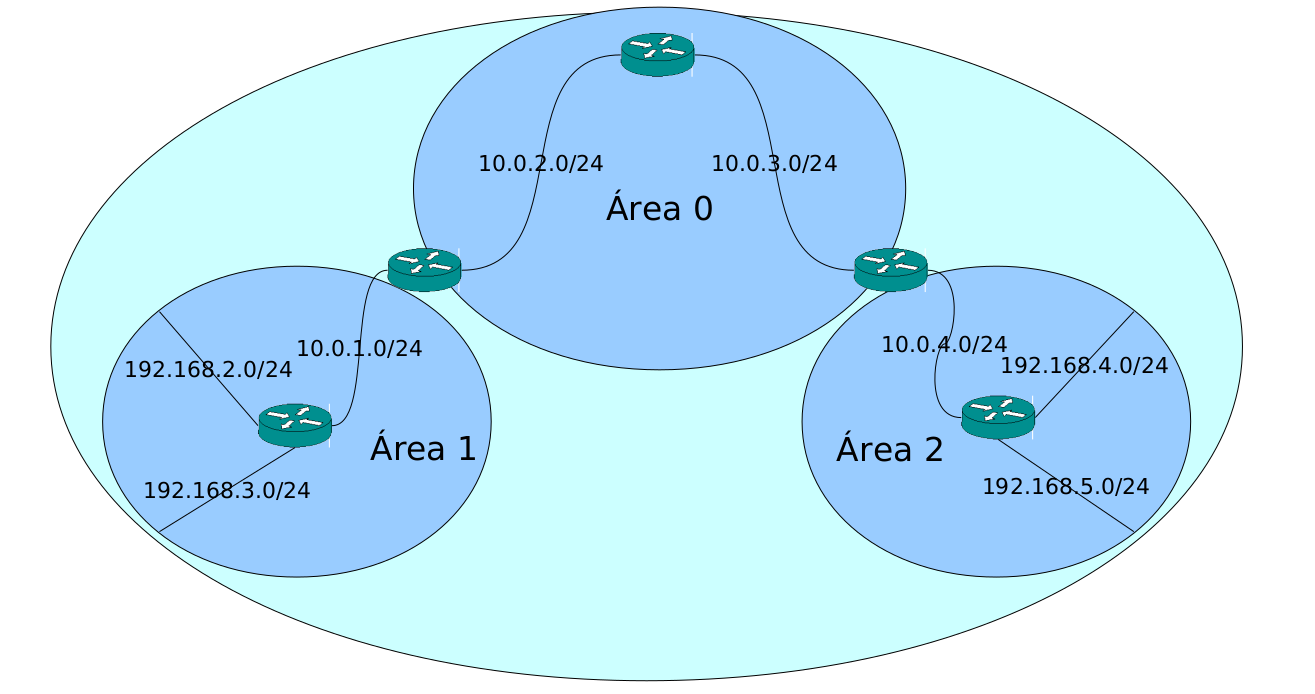
\includegraphics[width=\textwidth]{ospfv2}

\begin{minted}{bash}
  # net.conf
  defsw br12 uml1.0 uml2.0
  defsw net1 uml1.1
  defsw net2 uml1.2
  defsw br23 uml2.1 uml3.0
  defsw br34 uml3.1 uml4.0
  defsw br45 uml4.1 uml5.0
  defsw net3 uml5.1
  defsw net4 uml5.2 
\end{minted}

\begin{minted}{bash}
  # En cuanto se inician las UML, editar el fichero /etc/quagga/daemons la línea
  ospfd=no
  # Por
  ospfd=yes
  # A continuación restart del servicio
  systemctl restart quagga
  # Verificar que se ospfd está corriendo
  systemctl status quagga
\end{minted}

\begin{minted}{lexer.py:IOSLexer -x}
 ! UML1 (zebra.conf)
 conf[igure] term[inal]
 int[erface] eth0
 ip address 10.0.1.1/24
 no shutdown
 quit
 int[erface] eth1
 ip address 192.168.3.1/24
 no shutdown
 quit
 int[erface] eth2
 ip address 192.168.2.1/24
 no shutdown
 quit
 ip forwarding
 exit
 write
\end{minted}
\begin{minted}{lexer.py:IOSLexer -x}
 ! UML2 (zebra.conf)
 conf[igure] term[inal]
 int[erface] eth0
 ip address 10.0.1.2/24
 no shutdown
 quit
 int[erface] eth1
 ip address 10.0.2.2/24
 no shutdown
 quit
 ip forwarding
 exit
 write
\end{minted}

\begin{minted}{lexer.py:IOSLexer -x}
 ! UML3 (zebra.conf)
 conf[igure] term[inal]
 int[erface] eth0
 ip address 10.0.2.1/24
 no shutdown
 quit
 int[erface] eth1
 ip address 10.0.3.1/24
 no shutdown
 quit
 ip forwarding
 exit
 write
\end{minted}

\begin{minted}{lexer.py:IOSLexer -x}
 ! UML4 (zebra.conf)
 conf[igure] term[inal]
 int[erface] eth0
 ip address 10.0.3.2/24
 no shutdown
 quit
 int[erface] eth1
 ip address 10.0.4.2/24
 no shutdown
 quit
 ip forwarding
 exit
 write
\end{minted}

\begin{minted}{lexer.py:IOSLexer -x}
 ! UML5 (zebra.conf)
 conf[igure] term[inal]
 int[erface] eth0
 ip address 10.0.4.1/24
 no shutdown
 quit
 int[erface] eth1
 ip address 192.168.4.1/24
 no shutdown
 quit
 int[erface] eth2
 ip address 192.168.5.1/24
 no shutdown
 quit
 ip forwarding
 exit
 write
\end{minted}

\begin{minted}{lexer.py:IOSLexer -x}
 ! UML1 ospf.conf
 conf[igure] term[inal]
 router ospf
 ospf router-id 0.0.0.1
 network 10.0.1.0/24 area 1
 network 192.168.2.0/24 area 1
 network 192.168.3.0/24 area 1
 area 1 stub
 passive-interface eth1 ! Las redes de usuario irán siempre como passive-interface
 passive-interface eth2
 end
 write
\end{minted}

\begin{minted}{lexer.py:IOSLexer -x}
 ! UML2 ospf.conf
 conf[igure] term[inal]
 router ospf
 ospf router-id 0.0.0.2
 network 10.0.1.0/24 area 1
 network 10.0.2.0/24 area 0
 area 1 range 10.0.0.0/8 not-advertise ! No advierte de este area en otras areas por ser ABR
 end
 write
\end{minted}

\begin{minted}{lexer.py:IOSLexer -x}
 ! UML3 ospf.conf
 conf[igure] term[inal]
 router ospf
 ospf router-id 0.0.0.3
 network 10.0.2.0/24 area 0
 network 10.0.3.0/24 area 0

\end{minted}

\begin{minted}{lexer.py:IOSLexer -x}
 ! UML4 ospf.conf
 conf[igure] term[inal]
 router ospf
 ospf router-id 0.0.0.4
 network 10.0.3.0/24 area 0
 network 10.0.4.0/24 area 2
 area 2 range 10.0.0.0/8 not-advertise ! No advierte de este area en otras areas por ser ABR
 end
 write
\end{minted}

\begin{minted}{lexer.py:IOSLexer -x}
 ! UML5 ospf.conf
 conf[igure] term[inal]
 router ospf
 ospf router-id 0.0.0.5
 network 10.0.4.0/24 area 2
 network 192.168.4.0/24 area 2
 network 192.168.5.0/24 area 2
 area 2 stub
 passive-interface eth1 ! Las redes de usuario irán siempre como passive-interface
 passive-interface eth2
 end
 write
\end{minted}

Comprobar las tablas de ospf con el comando

\begin{minted}{lexer.py:IOSLexer -x}
 show ip ospf database
\end{minted}

\newpage
\section{OSPFv3}
Configurar 5 máquinas virtuales para crear el siguiente AS:

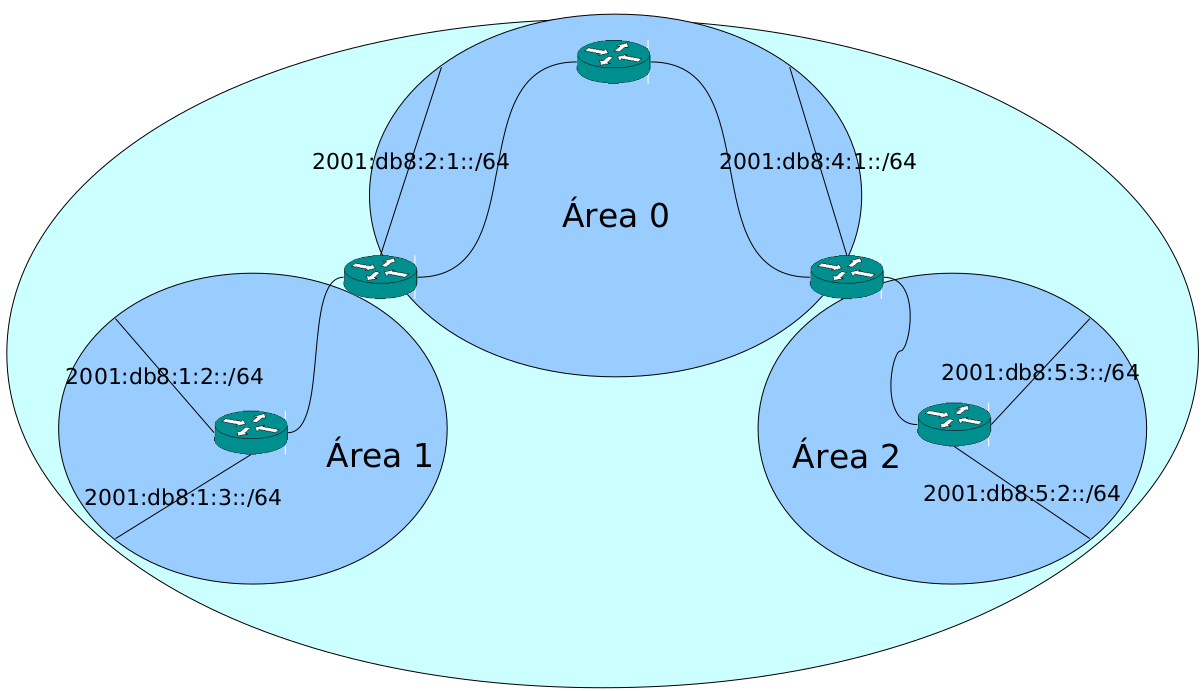
\includegraphics[width=\textwidth]{ospfv3}

\end{document}

